%lualatex fileName.tex
\documentclass[9pt]{ltjsarticle}
\usepackage{bm}
\usepackage{amsmath,amssymb}
\usepackage{tcolorbox}
\usepackage{graphicx}
\usepackage{booktabs}
\usepackage{subcaption}
\usepackage{tikz}
\usetikzlibrary{graphs,graphs.standard,graphdrawing}
\usegdlibrary{trees,force,layered}
\begin{document}
\title{TravelingSalesmanProblem}
\author{MunechikaHaruki}
\maketitle

\part{TSP}
\setcounter{tocdepth}{3}
\tableofcontents

\newpage
\section{最適化問題とは}
目的関数をいくつかの制約条件の元で最適化(最大化、最小化)する問題。

\subsection{線形計画問題の種類}
\begin{description}
    \item[線形計画問題] 目的関数が線形かつ、制約条件が線形線形の不等式または等式であるもの
    \item[非線形計画問題] 線形計画問題から、線形の制約を外したもの
    \item[ネットワーク計画問題] ネットワークで表現できる最適化問題
    \item[整数問題] 変数の中に、整数の範囲の定義域となるものがある問題
\end{description}
\subsubsection{線形計画問題はどのような形か}
\begin{tcolorbox}[title=線形計画問題の標準形]
    \begin{gather*}
        \text{目的関数}:\bm{c}^\top \bm{x}
        \longrightarrow \text{最小}\\        
        \text{制約条件}:\bm{Ax}=\bm{b},\bm{x} \ge \bm{0}
    \end{gather*}
\end{tcolorbox}
\subsubsection{最短路問題（TSPとおなじネットワーク計画問題）について述べよ}
\begin{figure}[h]
    \caption{ネットワークの例}
    \begin{center}
        \begin{tikzpicture}[line width=1.3pt,node distance=2cm]
            \node                    (a)[draw,circle]{$a$};
            \node[above right of= a ](b)[draw,circle]{$b$};
            \node[below right of= a ](c)[draw,circle]{$c$};
  %          \node[right of= a,node distance=3.62cm ](d)[draw,circle]{$d$};
            \node[      right of= b ](e)[draw,circle]{$e$};
            \node[      right of= c ](f)[draw,circle]{$f$};
            \node[right of= a,node distance=7.24cm ](g)[draw,circle]{$g$};
        
            \draw[->](a) -- (b)node[midway,above]{$5$};
            \draw[->](a) -- (c)node[midway,below]{$4$};
        
        
     %       \draw[->](b) -- (d)node[midway,above]{$4$};
            \draw[->](b) -- (e)node[midway,above]{$7$};
        
         
     %       \draw[->](c) -- (d)node[midway,above]{$6$};
            \draw[->](c) -- (f)node[midway,above]{$8$};
        
     %       \draw[->](d) -- (e)node[midway,above]{$5$};
     %       \draw[->](d) -- (f)node[midway,above]{$3$};
        
        
            \draw[->](e) -- (g)node[midway,above]{$3$};
        
        
            \draw[->](f) -- (g)node[midway,above]{$2$};
        
            \draw[->](b) to[bend right] node[midway,left]{$2$}(c);    
            \draw[->](c) to[bend right] node[midway,left]{$2$}(b);
            \draw[->](f) to[bend right] node[midway,left]{$2$}(e);   
            \draw[->](e) to[bend right] node[midway,left]{$1$}(f);
        
    \end{tikzpicture}
    \end{center}
    \end{figure}
    ネットワークを交通機関の路線とみなし、
    枝の横に書かれている数値をその路線を利用したときの所要時間とみなす。
    
    このとき、あるノードから別のノードへの路のうち、
    最小の所要時間を持つ路を選ぶのが最小路問題である。
    
    以下のように定式化できる。

    \hrulefill
    
    0-1条件を以下のように定義する。
    \begin{tcolorbox}[title=0-1条件]
        \begin{equation}
            x_{ij}=\begin{cases}
                1 , \text{(i,j)を通る}\\
                0 , \text{(i,j)を通らない}
            \end{cases}
        \end{equation}
    \end{tcolorbox}
    路(i,j)が持つ数値を$a_{ij}$とおく。すると、
    目的関数は、
    \begin{equation}
        \sum_{(i,j)} a_{ij}x_{ij}
    \end{equation}
    と書ける。この目的関数を以下の制約条件の元で
    最小化するのが最短路問題である。
    
    制約条件は、0-1条件で、枝が出ていく数
    と枝が入る数がちょうどよくなるように設定する。
    
\newpage
\section{TSPとは}
セールスマンが会社を出発して、いくつかの都市を訪問し、会社に
戻ってくる経路の中で、最良の経路を見つける問題である。
客の都市は必ず少なくとも一度は訪問しなければならない。

グラフ理論の言葉で言うと、ハミルトン閉路を求める問題である。

\subsection{TSPの定式化を行え}
\begin{tcolorbox}[title=巡回セールス問題の定式化]
    n個のノードを訪問することにする。ノードの集合を$V:={0,1,\dots,n-1}$
    とする。(ただし、$n>3$)

    全ての経路の集合を$E:=\{(i,j)|i,j\in V,i\neq j\}$と定義。

    経路(i,j)の距離を$d_{i,j}$と定義$(d_{ij}=d_{ji})$

    \begin{equation}
        x_{ij}:=\begin{cases}
            1 (\text{i番目のノードからj番目のノードを通る時})\\
            0 (\text{i番目のノードからj番目のノードを通らない時})
        \end{cases}
    \end{equation}
    \begin{align}
        \text{目的関数：}&\sum_{(i,j)\in E}d_{ij}x_{ij}\longrightarrow min\\
        \text{制約条件：}&\sum_{j\in V}x_{ij}=1,i\in V(ノードiから出るのは一本)\\
        &\sum_{i\in S}\sum_{j\in S}x_{ij}\le |S|-1,S\subset V\\
        &x_{ij}\in \{0,1\},(i,j)\in E(0-1\text{条件})
    \end{align}
\end{tcolorbox}
\subsection{TSPはどのような種類の問題に属するか}
 TSPはネットワークを用いた問題であるので、ネットワーク問題である。

 また、実行可能集合は$x_{ij}$が0-1変数であることから有限個
 の要素からなる。よって、TSPは組み合わせ計画問題
 (組み合わせ最適化問題)でもある。

 \subsection{TSP問題の難しさについて説明せよ}
 TSP問題は、NP完全であることが知られている。

 すなわち、多項式時間アルゴリズムのみつかっていないクラスNP
 問題のうち、最も難しい問題である。

 すなわち、もし問題を解く多項式時間アルゴリズム
 が存在するならば、クラスNPの中の全ての問題に
 その問題を解く多項式時間アルゴリズムの存在が保証されるということである。

 TSPと同じ多項式時間アルゴリズムの例として、充足性判定問題、
 ナップザック問題などがある。

 NP完全問題に対し多項式時間アルゴリズムを発見するのは
 非常に難しいので、
 次善のアプローチとして、近似アルゴリズムやヒューリスティクスがある。
 
 近似アルゴリズムとは最適解に対し、ある程度の範囲の誤差
 を持つ近似解を保証するアルゴリズムで、
ヒューリスティクス（発見的手法）とは、精度の保証はないが、
少ない計算量である程度の解が得られることが経験的に知らされている
アルゴリズムである。

本レポートでは、メタ・ヒューリスティクスの解法の一つである
遺伝的アルゴリズムでTSPを解く。

 \newpage
 \section{遺伝的アルゴリズム(GeneticAlgorithm)による巡回セールスマン問題の一解法}
本節では、TSP問題の近似アルゴリズムの一例として、遺伝的アルゴリズム(
    以下GAと略
)による巡回セールスマン問題の一解法を
用いる。以下に、その詳細を示す。
\subsection{遺伝的アルゴリズムとはなにか}
\begin{tcolorbox}[title=遺伝アルゴリズムの概要]
GAは、自然界における生物進化のモデル化である。

個体群の中で、環境への適応度の高い個体を選択し、
交叉および突然変異を起こしながら次の世代を形成していく過程を用いた
メタ・ヒューリスティクスである。

TSPに対する適用以外でも、機械学習などに対する分野でも
幅広い活躍を見せている。

\end{tcolorbox}
\subsection{枝交換交叉のやり方について述べよ}
\begin{tcolorbox}[title=TSPの解の染色体への符号化]
    TSPの解の染色体への符号化として、
    ノード$V:={A,B,C,D,E,F}$のとき、
    \begin{align*}
        \begin{matrix}
            AB&BC&CE&ED&DF&FA\\
        \end{matrix}
    \end{align*}
    のように、連続して訪問する都市の対を
    巡回すべきと数だけ並べた染色体を用いる。

    ここでの都市の対をマクロ遺伝子、
    左からi番目のマクロ遺伝子を遺伝子座iのマクロ遺伝子と呼ぶことにする。

    マクロ遺伝子ABがあったとして、
    Aを第一コドン、Bを第２コドンと呼称する。
\end{tcolorbox}
   生物は次世代へと子孫をつなげる時、父親と母親の遺伝子を混ぜ合わせる。
    これを交叉という。

    この問題において
    交叉とは、２つの染色体の遺伝子を一部交換することで、
    親個体より良い個体を生成することを示す。

    交叉に相当する演算には様々なものが提案されているが、今回は
    枝交換交叉を用いる。

    以下に、枝交換交叉のアルゴリズムを示す。
\begin{tcolorbox}[title=交叉に相当する操作]
\begin{enumerate}
    \item 全ての個体をランダムにペアリングし、各ペアに親１、親２とラベル分けする
    \item 親1でランダムにマクロ遺伝子を選びその遺伝子座を$i_1$とする
    \item 遺伝子座$i_1$のマクロ遺伝子の第一コドンと同じ第一コドンを持つ親２
    のマクロ遺伝子の遺伝子座を$i_2$とする。
    \item $i_1$、$i_2$の第二コドンと、もう一方の親の第一コドン
    が等しければ、それぞれと対応付け、その遺伝子座を$j_1,j_2$
    とする。
    \item $i_1,i_2$のマクロ遺伝子をを交換する
    $i_1,i_2$の第二コドン同士が等しければ終了
    \item $i_1,i_2$の後に$j_2,j_1$が来るように
    $j_2,j_1$遺伝子をもってくる。
    \item $j_1\rightarrow i_1,j_2
    \rightarrow i_2$として(3)
    に戻る
\end{enumerate}
枝交換交叉では、第二コドンの等しい枝の交換が行われるまで枝の交換が
続く。
\end{tcolorbox}

\subsection{突然変異のやり方を一つ述べよ}
\begin{tcolorbox}[title=突然変異に相当する操作]
    交叉が成立しなかった個体(
        遺伝子の交換が行われなかった個体
    )に対して、突然変異を行う。

    操作として、順回路の一部を逆順にする操作を行う。

    \begin{enumerate}
        \item ランダムに２つのマクロ演算子を選択
        \item 2つのマクロ演算子の第一コドンと第二コドンの間
        で染色体を分割し、染色体をさん分割する
        \item 分割された染色体の中央部を逆順にする
    \end{enumerate}
\end{tcolorbox}

\subsection{TSPの最適化の流れを述べよ}
\begin{tcolorbox}[title=適応と選択]
    ある世代から次の世代の個体がN体生み出されたとする。
    この時、親と比べて、優秀な個体(総経路が短い)
    や劣った個体が生まれるはずである。(総経路が長い)

    この「優秀さ」の評価指標を\textbf{適応度}と呼ぶ。

    順回路長lに対し、適応度$f(l)$を
    少しの違いでも大きな差が現れるように、冪乗則を用い
    \begin{equation}
        f(l):=(\frac{n}{l})^3
    \end{equation}
    と定義する。

    子世代から、適応度の高い個体を選択する。

    ただ、適応度が高い順にただ選択するだけでは、
    遺伝的多様性が失われ、局所最適に陥る危険性がある
    ことに注意する。
\end{tcolorbox}

以上で、交叉演算と突然変異演算を定義した。
次に、これらを組み合わせて実際に最適化を行うまでの
流れを示す。
\begin{tcolorbox}[title=最適化までの流れ]
\begin{enumerate}
    \item N個の個体をランダムに生成する。
    \item それぞれの個体の適応度を計算する
    \item 新たに親となるn個$(n<N)$を適応度の高い順に選択する
    \item n個の個体からランダムにペアを作り、そのペアから
    子を新たにN体作る
    \item 確率で突然変異させる
    \item (2)に移動
\end{enumerate}
世代交代のは、各世代の適応度の
最大値を記録し、その変化が少なくなった時に打ち止める。
\end{tcolorbox}


\newpage
\section{枝交換交叉によるGAでの巡回セールスマン問題の実装}
上の章で示されたアルゴリズムに基づき、C言語で
\verb|solve_GeneticAlgorithm|関数を実装した。
それを以下に示す。

\begin{center}
    \begin{verbatim}
        //*遺伝的アルゴリズム(GA) ある程度以上の最適化に弱い*//
        double solve_geneticAlgorithm(int p[],double d[N][N],int n)
        {
          int generationNum=10000000;//世代の数
          int eliteNum=ELITENUM;//親の数
          int numOfIndivisuals=MAXINDIVIDUAL;//世代の個体の数
          double normPathLength=NORMPATHLENGTH;
          double percentOfMutation=MUTATE;
          int Individual[MAXINDIVIDUAL][N];//個体の経路を記録
          int newIndividual[MAXINDIVIDUAL][N];//子世代の個体の経路を記録
          double Fitness[MAXINDIVIDUAL],totalPath[MAXINDIVIDUAL];//個体ごとの適応度、総経路を記録
          int suffixOfFitness[MAXINDIVIDUAL];//tatalPathに付けられた添字で、今何番目かを記録
          int MotherRank,FatherRank;//親となる個体の順位
          int Mother[N],Father[N],Child[N];//親と子の経路
          double bestPathLength=100000000;
        
        
          //初期化
          InitializeIndividuals(Individual,n,numOfIndivisuals);
          for(int k=0;k<numOfIndivisuals;k++)
            totalPath[k]=bestPathLength;
        
          for(int g=0;g<generationNum;g++){
          //合計、適応度の計算
          calcTotalroute(Individual,d,n,numOfIndivisuals,totalPath);
          calcFitness(totalPath,numOfIndivisuals,Fitness);
          //添字の初期化
          for(int i=0;i<numOfIndivisuals;i++){
            suffixOfFitness[i]=i;
          }
        
          //添字をソート
          sortSuffix(Fitness,suffixOfFitness,numOfIndivisuals);
         
          //現世代での最高適応度の個体を記録  
          printf("generation:%d :%lf\n",g,totalPath[suffixOfFitness[0]]);
          if(totalPath[suffixOfFitness[0]]<bestPathLength){
            bestPathLength=totalPath[suffixOfFitness[0]];
          for(int i=0;i<n;i++){
            p[i]=Individual[suffixOfFitness[0]][i];
          }
          }
        
          //親の選択と次世代の個体の生成
          for(int i=0;i<numOfIndivisuals;i++){
            MotherRank=rand()%eliteNum;
            FatherRank=rand()%eliteNum;
            for(int j=0;j<n;j++){
              Father[j]=Individual[suffixOfFitness[FatherRank]][j];//ここなにかある
              Mother[j]=Individual[suffixOfFitness[MotherRank]][j];
            }
            createChild(Father,Mother,Child,n);
            if(rand()/RAND_MAX<percentOfMutation)mutation(Child,n);
        
            for(int j=0;j<n;j++){
              newIndividual[i][j]=Child[j];
            }
          }
          //世代交代
          for(int i=0;i<numOfIndivisuals;i++)
            for(int j=0;j<n;j++)
              Individual[i][j]=newIndividual[i][j]; 
        
            if(bestPathLength<normPathLength){
              save_path("mk_neighbor.path", p,n);
              break;
            }
          }
          return bestPathLength;
        }
    \end{verbatim}
\end{center}

本章では、この関数\verb|solve_geneticAlgorithm|について解説する。

\begin{tcolorbox}[title=GeneticAlgorithmソルバ]
\begin{verbatim}
double solve_geneticAlgorithm(int p[],double d[N][N],int n)
\end{verbatim}
\begin{description}
    \item[p]TSPの解となる経路
    \item[d]ノード同士の距離を表す距離行列
    \item[n]ノードの数
    \item[返り値]GAで求められたTSPの解の総経路長
\end{description}

\hrulefill

ここでは\verb|solve_geneticAlgorithm|の内部変数について解説する

()の中は変数の型を示す。
\begin{description}
    \item[generationNum]世代の最大数。世代がこの数を超えると強制終了する(int)
    \item[eliteNum]適応度の高い順に選ばれる親の候補の数(int)
    \item[numOfIndividuals]世代ごとの個体の数(int)
    \item[normPathLength]経路長のノルマ。最小の経路長を持つ個体の
    経路長がこの数より小さくなると終わる(double)
    \item[percentOfMutation]生まれてきた子供の突然変異の確率(double)
    \item[Individual]行に個体ごとの経路情報を格納(int [ ][ ])
    \item[newIndividual]individualから作られた
    新しい世代の経路情報を格納(int [ ][ ])
    \item[Fitness]totalPathから適応度を計算し、格納するための配列(double [ ])
    \item[totalPath]Individualとdから個体ごとに計算された
    個体ごとの総経路長を格納(double [ ])
    \item[suffixOfFitness]Individualの個体ごとに付けられる
    添字。totalPathと一緒に降順にソートされ、適応度の高い個体を選択する
    際にも使われる。(int [ ])
    \item[Mother,Father,Child]2つの親と子個体の経路情報を
    格納するための配列(int [ ])
    \item[bestPathLength]これまで作り出された個体の中での最短経路
    を記録(double)
\end{description}
\end{tcolorbox}

このGAソルバは複数の関数に依存している。ここではその
依存関係を上から下への階層構造として、以下に示す。

\tikzset{my node/.style={circle}}
\begin{center}
\begin{tikzpicture}
    \graph[layered layout]{
        GeneticAlgorithm -> 
        {InitializeIndividual,calcTotalroute,
        calcFitness,sortSuffix,createChild
        ->{encodeChromosome,decodeChromosome,
        reverseChromosomePart
        ->{reverseArrayPart->{reverseArray}}},
        savePath}
    };
\end{tikzpicture}
\end{center}
次に、上にあるようなGeneticAlgorithmソルバの内部で使われる
関数について説明する。

これらの関数の実装方法については本レポートの中では解説しない。
簡単な機能のみに絞る。引数と戻り地については実際のプログラム内を参照
\begin{tcolorbox}[title=GeneticAlgorithmソルバの内部関数]
\begin{description}
    \item[InitializeIndividual]Individual配列に対し、行ごとに
    0~(ノード数-1)を被りなくランダムに敷き詰める関数
    \item[calcTotalroute]Individual配列と距離行列dから、
    行ごとの総経路長を計算し、配列totalPathに格納
    \item[calcFitness]配列totalPathから適応度を計算し
    結果を配列Fitnessに代入
    \item[sortSuffix]FitnessとsuffixOfFitnessを指定すると、
    Fitnessが降順になり、それと同じようにsuffixOfFitnessも入れ替える。
    (個体番号を適応度が大きい順にソートする関数)
    \item[createChild]2つの親を指定することで子供を作る関数
    \item[savePath]経路を保存する関数
    \item[encodeChromosome]経路を染色体にする関数
    \item[decodeChromosome]染色体を経路にする関数
    \item[reverseChromosomePart]染色体と適当な数i,jを指定すると、
    第i座と第j座の間にある全ての遺伝子を逆順にする関数
    \item[reverseArrayPart]配列を部分的に逆順にする関数
    \item[reverseArray]配列を逆順にする関数
\end{description}
\end{tcolorbox}

次に、関数内での大まかな処理の流れを以下に示す。
\begin{center}
    \begin{tikzpicture}
        \graph[layered layout]{
            Initialize関数で初期化 -> 
            個体ごとの経路長の合計、適応度の計算 ->
            添字の初期化 ->
            添字のソート　->
            親の選択と次世代の個体の生成 ->
            世代交代〔newIndividualをIndividualに代入〕 ->
            個体ごとの経路長の合計、適応度の計算
            
        };
    \end{tikzpicture}
\end{center}

elitefNumなどのハイパラメータに代入されている
NやMAXINDIVIDUALは、オブジェクト形式マクロである。

遺伝的アルゴリズムはその性質上、ハイ・パラメータの探索
が必須である。

ハイパラメータは一度に変えるのが望ましいため、
オブジェクト形式マクロとしてプログラムの先頭で一気に扱うことにした。

実行時には、プログラムの頭で定義されたオブジェクト形式マクロを
変化させながら、局所最適に陥らずより良い解が得られるような
値を探索する。

下に、実行時にオブジェクト形式マクロ一覧を示す。
\begin{tcolorbox}[title=プログラム中のオブジェクト形式マクロ一覧]
\begin{description}
    \item[N] ノードの最大数
    \item[MAXINDIVIDUAL] 個体の数
    \item[NORMPATHLENGTH] ノルマとなる経路長(これより短い経路がでてくればループが終了)
    \item[MUTATE] 変異率
    \item[ELITENUM] 親の数
\end{description}
\end{tcolorbox}
\begin{tcolorbox}[title=プログラムの実行例]
ハイパラメータとして、
世代ごとの個体数1000、変異率0.8、親の数7、総経路のノルマを450で与える
座標データをdata20
とする。このときの実行結果のうち、\verb|solve_geneticAlgorithm|
関数による標準出力の部分を以下に示す。

\hrulefill
\begin{verbatim}
generation:0 :1330.617481
generation:1 :1222.243377
generation:2 :1104.233158
generation:3 :994.046342
...(中略)
generation:28 :483.928012
generation:29 :481.001254
generation:30 :471.553964
generation:31 :465.178237
generation:32 :455.875895
generation:33 :455.010522
generation:34 :449.828530
\end{verbatim}
これを見れば、\verb|solve_geneticAlgorithm|
は妥当な近似解を出力できることがわかる。
\end{tcolorbox}



\newpage
\section{コンテストのデータを用いた結果}
コンテストで用いたdata20,data21,data22に対し、
上のGeneticAlgorithmソルバを適用させ、
近似解を得た。

以下にそうして得られた経路の図を二通り、そしてその総経路長、またその時に
使ったハイパラメータ(総経路のノルマ以外)を図のキャプションに示す。

コンテスト時に得られたデータが残っていないので、実行し直したことを追記
する。
\begin{figure}[h]
    \centering
    \caption{data20}
    \begin{subfigure}{0.4\columnwidth}
        \centering
        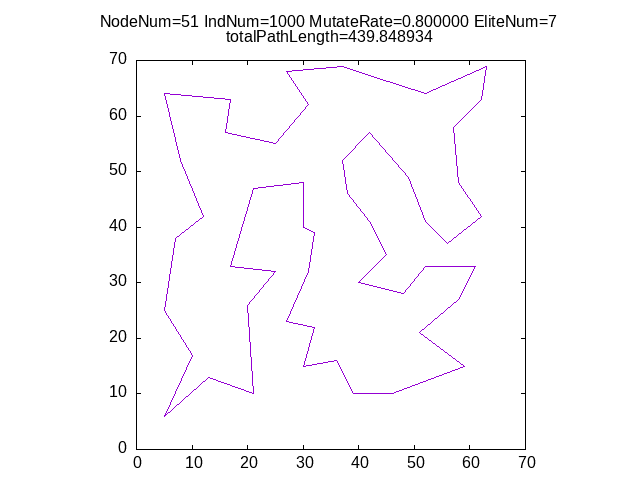
\includegraphics[width=\columnwidth]{data20a.txt.png}
        \caption{総経路長：439.848934}
    \end{subfigure}
    \centering
    \begin{subfigure}{0.4\columnwidth}
        \centering
        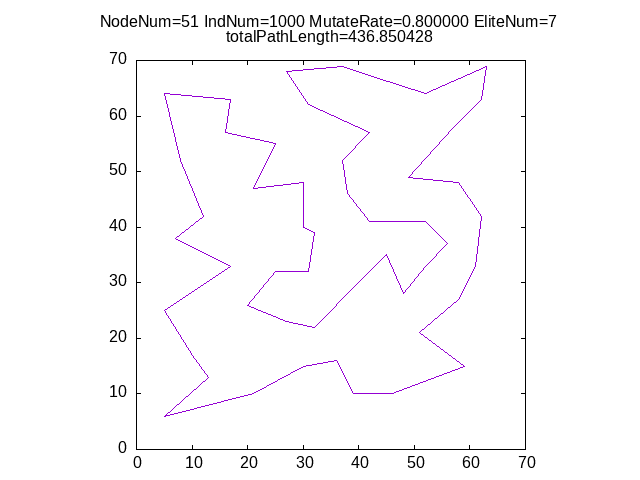
\includegraphics[width=\columnwidth]{data20b.txt.png}
        \caption{総経路長：436.850428}
    \end{subfigure}
\end{figure}
\begin{figure}[h]
    \centering
    \caption{data21}
    \begin{subfigure}{0.4\columnwidth}
        \centering
        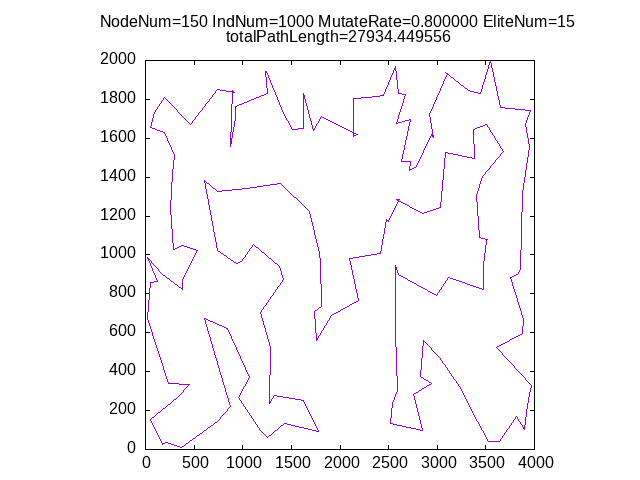
\includegraphics[width=\columnwidth]{data21a.txt.png}
        \caption{総経路長：27934.449556}
    \end{subfigure}
    \centering
    \begin{subfigure}{0.4\columnwidth}
        \centering
        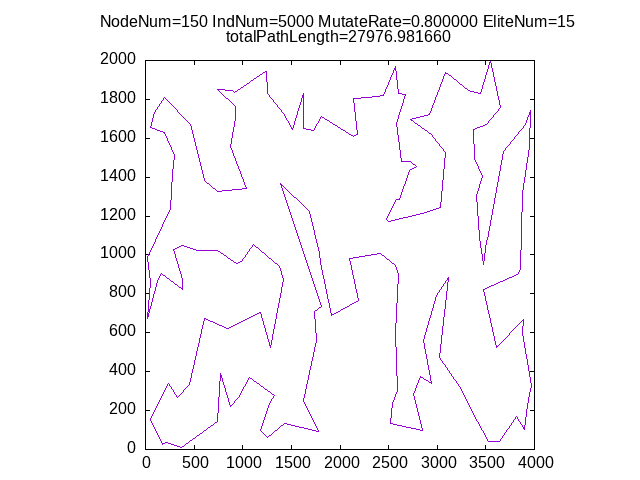
\includegraphics[width=\columnwidth]{data21b.txt.png}
        \caption{総経路長：27976.981660}
    \end{subfigure}
\end{figure}
\begin{figure}[h]
    \centering
    \caption{data22}
    \begin{subfigure}{0.4\columnwidth}
        \centering
        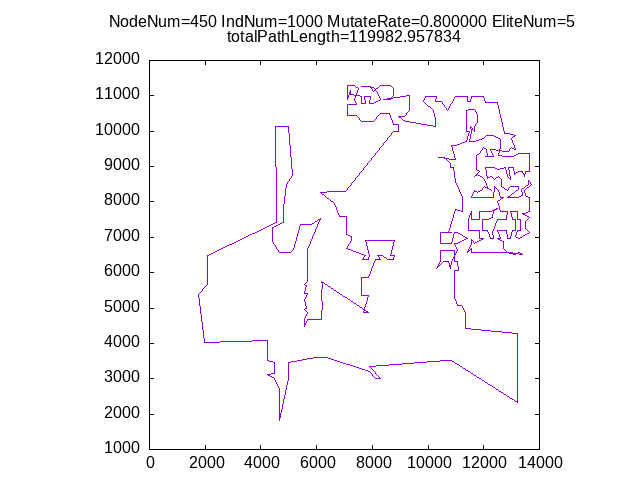
\includegraphics[width=\columnwidth]{data22a.txt.png}
        \caption{総経路長：119982.957834}
    \end{subfigure}
    \centering
    \begin{subfigure}{0.4\columnwidth}
        \centering
        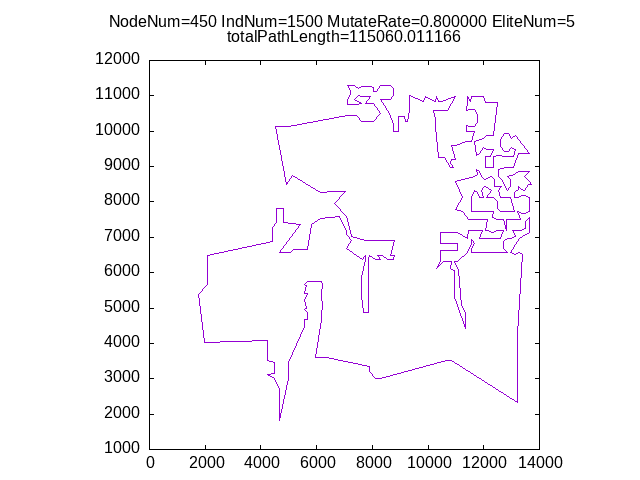
\includegraphics[width=\columnwidth]{data22b.txt.png}
        \caption{総経路長：115060.011166}
    \end{subfigure}
\end{figure}
\newpage
\subsection{手法の特徴と結果についての考察}
遺伝的アルゴリズムは、ある程度までの近似解を得ることは得意だが、
最適解やほぼ限りなく最適解に近い近似解を得ることが難しい
アルゴリズムである。
このことは、data21とdata22のコンテストでの順位が、
90人中30位程度だったことからも見て取れる。

原因として、遺伝的アルゴリズムそのものが、計算量に応じて
解の収束を保証しないヒューリスティクスなアルゴリズムである
ことが考えられる。

それと同時に、GAは、複数のハイパラメータを設定しないといけない
ため、扱いが難しいアルゴリズムでもある。
実際にdata20のコンテストの順位は、ハイパラメータの最適化不足
でほぼ最下位になってしまった。

ハイパラメータそのものを最適化するようなアルゴリズムも考案されているが、
あまり普及していない。
TSPのような研究が進んでいる問題を解く際には、GAなどの
ヒューリスティクス解法ではなく収束が保証されている
近似アルゴリズムを使用するべきである。

\end{document}